\section{When splitting is safe, and what it costs}
\label{sec:safe}

Splitting cannot lower expected recall when no view zooms out and views overlap by one object, and neither part can be dropped. Every such split pays a minimum cost, and our rule pays it up to an explicit factor. All data show both predictions (\cref{fig:map}), and the guarantee fails exactly at the two places the theory names.

\paragraph{What the caller controls and what is tested.} A call $c$ shows a rectangular view $V_c$ of a source image at scale $s_c$, keeps the returned points inside a core $K_c \subseteq V_c$, and uses a fixed prompt. A target is \emph{interior} to $c$ if its box lies in $V_c$ and its centre at least $\tau$ inside $K_c$; $J_c$ is the set of interior centres. A \emph{model} gives a response law $P_X(\cdot \mid c)$ for every image $X$ and call $c$. For a distribution $\mathcal{D}$ of images (an application, a benchmark, or one image), a weight $a(X) \ge 0$ and a region $U$, $\nu_c(U) = \mathbb{E}[a(X) \sum_{x \in Y(X) \cap U \cap J_c} H_c(x)]$, where $Y(X)$ holds the target centres and $H_c(x) = 1$ if $c$ returns a kept point within $\tau$ of $x$; $a = 1$ counts detections, $a = 1/n(X)$ gives mean recall per image, and every result below holds for each $a$. A call $c'$ is a \emph{crop} of $c$ if it shows a sub-region of the same pixels at $s_{c'} \ge s_c$, and it \emph{refines} $c$ if it shows the same region at $s_{c'} \ge s_c$. The caller controls the geometry: no view zooms out, and views overlap by one object. The behaviour of the model is assumed, and tested:

\par\noindent\begin{minipage}{\linewidth}
\begin{assumption}[Monotonicity]
\label{ass:mono}
For all calls $c, c'$ and every region $U \subseteq J_c \cap J_{c'}$: (R) if $c'$ refines $c$, then $\nu_{c'}(U) \ge \nu_c(U)$: more tokens per target do not hurt; (M) if $c'$ is a crop of $c$ at the same scale, then $\nu_{c'}(U) \ge \nu_c(U)$: less content does not hurt.
\end{assumption}
\end{minipage}

$\mathcal{M}_{R,M}$ denotes the models satisfying Assumption~\ref{ass:mono}, whose two properties are averages that an experiment can estimate (zoom tools need one more property, \supp{A}).

\subsection{The exact condition for protection}

\begin{theorem}[Safe splitting]
\label{thm:safe}
Let the whole-image call show the image at $\Sw$, and let views $c_1, \dots, c_k$ be crops of it, so that $S_i \ge \Sw$. Under (R) and (M), if the cores shrunk by $\tau$ cover the image shrunk by $\tau$ and each view extends its core by half a target box on each side, the views together detect, in expectation, at least as many of the targets interior to the whole-image call as it does. This sufficient construction fixes the cores first and then adds the margin; in its terms, adjacent cores overlap by one target.
\end{theorem}

\Cref{thm:safe} establishes safety; \cref{thm:exact} gives the exact criterion and the cost lower bound; \cref{cor:safe} gives a construction within an explicit factor of it.

\begin{theorem}[Exact condition and minimum cost]
\label{thm:exact}
Let $\mathrm{d}$ be any finite set of calls. (a) If every centre interior to the whole-image call is interior to some call of $\mathrm{d}$ that is a crop or a refinement of it, then under (R) and (M), $\mathrm{d}$ detects in expectation at least as many of the targets interior to the whole-image call as it does, for every $\mathcal{D}$. (b) If target centres are more than $2\tau$ apart and some location interior to the whole-image call is interior to no such call, there is a $P \in \mathcal{M}_{R,M}$ under which the whole-image call detects every target interior to it and $\mathrm{d}$ never detects a target there. (c) If every interior centre is interior to such a call with $S_c \ge S \ge \Sw$, these calls use at least
\[
\Cmin = |J_{\mathrm{w}}|\,\lambda/(1 - \sigma)^2
\]
tokens, whatever the shapes, sizes, cores and overlaps of their views, where $|J_{\mathrm{w}}| = (W - e_x)(H - e_y)$ with margins $e_x = \max(w, 2\tau)$, $e_y = \max(h, 2\tau)$, $\lambda = S^2/m^2$ tokens per native pixel, and $\sigma = \sqrt{\lambda e_x e_y / N} < 1$.
\end{theorem}

\begin{proposition}[Each part is necessary]
\label{prop:tight}
For targets more than $2\tau$ apart: (a) if a target lies in the core of no view with $S_i \ge \Sw$, some $P \in \mathcal{M}_{R,M}$ makes the whole-image call find every target interior to it and the split never find that one; (b) neither (R) nor (M) can be dropped: for each, a model satisfying the other loses every target under some split while the whole-image call finds every target interior to it.
\end{proposition}

Protection is thus decided location by location: call a crop or refinement of the whole-image call \emph{qualified}; a split is protected for every model in $\mathcal{M}_{R,M}$ exactly when the interior set of the whole-image call satisfies \mbox{$J_{\mathrm{w}} \subseteq \bigcup\nolimits_{i \in I_{\mathrm{qual}}} J_i$}, the union over its qualified views (for targets more than $2\tau$ apart). A view that zooms out is not qualified, and never zooming out, with one object of overlap, meets the criterion. The same condition protects every local task with one position and one answer per object (\supp{A}).

\subsection{The minimum cost, and a rule within a factor of it}

\begin{algorithm}[t]
\caption{Safe splitting near the minimum cost}
\label{alg:rule}
\begin{algorithmic}[1]
\Require image $W \times H$, target box $w \times h$, interface ($t$, $N$ or $g$), protection point $S^\ast$
\State $S \gets \max(S^\ast, \Sw)$ \Comment{never zoom out}
\State cut the image at scale $S$ into the largest views within the budget, overlapping by $e_x$ and $e_y$, each its own core ($K_i = V_i$) and sent without further resizing
\State \emph{optional:} if a view holds many targets or busy content, also send sub-views of it at the same scale, overlapping by one target, and keep the view's points too (a subdivision fixed in advance for every view may instead replace the views)
\State send each view; keep its points, map them back and return them all, without merging duplicates
\end{algorithmic}
\end{algorithm}

\begin{corollary}[A safe split near the minimum]
\label{cor:safe}
Steps 1 and 2 of \cref{alg:rule}, with views $a_x \times a_y$ at pitches $p_x = a_x - e_x$ and $p_y = a_y - e_y$, detect in expectation at least as many of the targets interior to the whole-image call as it does under (R) and (M), and use at most $\Gamma\,\Cmin$ tokens, $\Gamma = \chi\,(1 + p_x/(W - e_x))(1 + p_y/(H - e_y))$, excluding per-image overhead. The rounding factor $\chi \ge 1$ equals 1 for ideal views of whole patches, for which the cost approaches $\Cmin$ as the image grows.
\end{corollary}

Hence $\Cmin \le C_{\mathrm{rule}} \le \Gamma\,\Cmin$ in image tokens, with $\Gamma$ set by the image, the target box, $S$ and the interface. Step 3 has two forms (\supp{I}). Sub-views \emph{appended} to a view cannot lower hits or matched true positives on any image, with no assumption, so the choice of which views to subdivide may depend on their content or answers; this form costs \CstepAppMin{} to \CstepAppMax{} times a view's tokens for resolution-scaled models (\CstepGridApp{} for fixed grids). Sub-views that \emph{replace} a view satisfy \cref{thm:exact}(a) when the subdivision is fixed in advance by the image's size, at \CstepRepMin{} to \CstepRepMax{} times its tokens. \Cref{tab:main} evaluates the rule without step 3.

\paragraph{Choosing the protection point.} $S^\ast = 1.5$ lies above the half-recall point of every model we tested, and \cref{cor:safe} holds for any $S^\ast$. The assumptions fix the sign of the gain, not its size:

\begin{proposition}[Attainable recall gains]
\label{prop:nonid}
Let target centres be more than $2\tau$ apart, with a continuous intensity. For any $0 \le r_{\mathrm{w}} \le r_{\mathrm{d}} \le 1$ some $P \in \mathcal{M}_{R,M}$ gives the whole-image call recall $r_{\mathrm{w}}$ and a covering split of \cref{thm:safe}, none of whose views is the whole image at the whole-image call's scale, recall $r_{\mathrm{d}}$ (weighted ratios of expected counts over the targets interior to the whole-image call).
\end{proposition}

Whether raising $S^\ast$ from 1.5 to 3 pays therefore depends on the model; at $S = \max(S^\ast, \Sw)$ it multiplies the area term of the cost by up to four (\cref{thm:exact}c); see \cref{fig:map}.

\subsection{Evidence across all data}

\begin{figure*}[t]
\centering
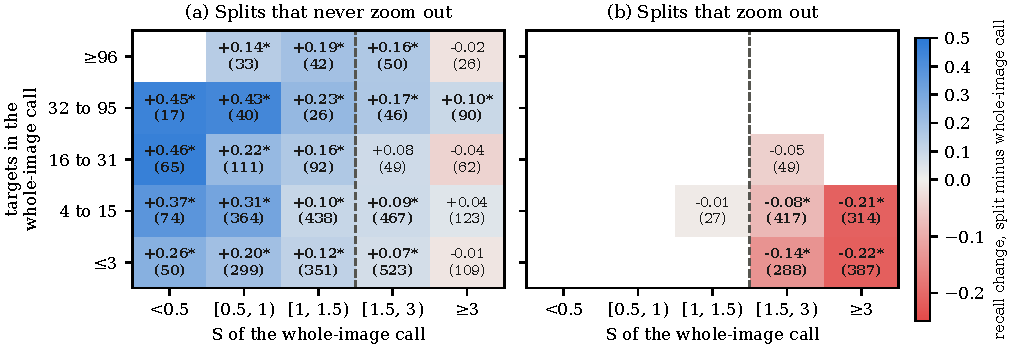
\includegraphics[width=\textwidth]{figures/fig3.pdf}
\caption{Where splitting helps and where it hurts. Mean recall change, split minus whole, over every pair of a whole-image call and a split in our data, binned by the whole-image call's $S$ and number of targets; pairs are grouped by geometry only (does any view zoom out?). Drawings and floor plans use the tiles of the 44 px recipe and its fixed-grid counterpart, natural images same-scale $2 \times 2$ tiles. Recall: matched recall over all targets of the image, pooled over the eight models (Gemini 3.8 at three budgets) and all 40 LegendSpot drawings, the six prompt-writing sheets included. The recipe's tiles do not overlap, so panel (a) checks the no-zoom-out part of the condition. Dashed line: $S = 1.5$. Pairs per cell in parentheses; blank: fewer than 10 pairs; ${}^\ast$: 95\% bootstrap interval excludes 0 (images resampled; mosaics by source drawing). Details in \supp{H}.}
\label{fig:map}
\end{figure*}

Both predictions show in all our data (\cref{fig:map}). \emph{Splits that never zoom out} gain: every cell with $S < 1.5$ gains significantly, and no cell is significantly below zero. The gain grows as $S$ falls, \CmapLowSMin{} to \CmapLowSMax{} for $S < 0.5$, and, once $S$ is ample, as targets multiply: for $S$ between 1.5 and 3 it rises from \CmapMidSMin{} to \CmapMidSMax. This band comes mainly from Gemini 3.8, Gemma, Qwen and Claude (\CmapBandMin{} to \CmapBandMax); the GPT models are near 0. \emph{Splits that zoom out} lose in every cell, by \CmapZoomMin{} to \CmapZoomMax, significantly in \CmapZoomSig{} of \CmapZoomCells.

\paragraph{Controlled test.} On 12 controlled $2{,}048^2$ images, 8 models and 5 relations, every pair of calls meets the definitions exactly. \XasSup{} of the \XasN{} orderings (pairs of calls whose detections the assumptions order) hold significantly and none is violated. At fixed $S$, safe tiles, with less content per call, raise recall by \XasThmMin{} to \XasThmMax, significantly for \XasThmSup{} of \XasModels{} models (\supp{F}). Of the \XtcN{} pairs of calls that the assumptions order in our other experiments, \XtcSup{} hold significantly and \XtcViol{} are violated (below).

\paragraph{Robustness and F1.} When the assumptions hold only approximately, the split's recall is at least the whole-image call's minus the measured (R) and (M) defects, the uncovered share and any loss from merging duplicates; no term grows with the number of views, and some model attains the bound. A split keeps F1 at least that of the whole-image call if and only if its added false points are at most $\rho_{\mathrm{w}} = (n + \mathrm{FP}_{\mathrm{w}})/\mathrm{TP}_{\mathrm{w}} \ge 1/\mathrm{Rec}_{\mathrm{w}}$ times its added hits, where $\mathrm{TP}_{\mathrm{w}}$, $\mathrm{FP}_{\mathrm{w}}$ and $\mathrm{Rec}_{\mathrm{w}}$ are the whole-image call's true positives, unmatched points and recall (\supp{A}).

\subsection{Where protection ends}

\paragraph{Boundary one: the assumptions fail.} The guarantee covers only input paths on which (R) and (M) hold: given more pixels of the same content, a model may process the input differently. All \XtcViol{} violations we found are of this kind, OpenAI models sent larger images than our standard input (one example in \cref{sec:intro}). Before trusting a new path, such as a high-resolution mode or uploading a large image at native size, a caller should test (R) with a few pairs of calls on the same region at different token counts, or split the image by the rule so that every view stays within the budget.

\paragraph{Boundary two: the condition fails.} A location that no qualified view covers is unprotected, and a view that zooms out is not qualified (\cref{thm:exact}b): the guarantee is gone. Tiling that first rescales the image to a pixel target zooms out whenever the whole image already gives $S$ above the recipe's, which depends on the image's size and is visible only by computing $S$ (\cref{fig:intro}c, \cref{fig:map}b). Choosing $S = \max(S^\ast, \Sw)$ excludes this by construction.
